\documentclass[aspectratio=169,10pt]{beamer}
\usepackage[utf8]{inputenc}
\usepackage[T1]{fontenc}
\usepackage{amsmath,booktabs,graphicx}
\usetheme{default}
\usefonttheme{professionalfonts}
\setbeamertemplate{navigation symbols}{}
\setbeamertemplate{footline}{\hfill\scriptsize\insertframenumber/\inserttotalframenumber\hspace{4mm}\vspace{2mm}}
\definecolor{ink}{HTML}{0B0B0B}\definecolor{accent}{HTML}{2A78D6}\definecolor{warm}{HTML}{EB6834}
\setbeamercolor{frametitle}{fg=ink}\setbeamercolor{structure}{fg=accent}\setbeamercolor{normal text}{fg=ink}
\setbeamerfont{frametitle}{series=\bfseries,size=\large}
\setbeamertemplate{itemize items}[circle]
\graphicspath{{../results/figures/}}
\newcommand{\tab}[1]{\input{../results/tables/#1.tex}}
\newcommand{\Rsq}{$R^2$}
\title{Attention-Infused Parallel ANFIS for Effluent BOD Prediction}
\subtitle{Re-implementation, reproduction on public data, and a stress test}
\author{Jack Emre Flett}
\institute{Fuzzy Logic (Bulan{\i}k Mant{\i}k) term project \\ Istanbul University-Cerrahpa\c{s}a, Computer Engineering}
\date{November 2026}
\begin{document}
\frame{\titlepage}

\begin{frame}{The problem: effluent BOD arrives five days too late}
\begin{columns}[T]
\column{0.56\textwidth}
\begin{itemize}\setlength\itemsep{2mm}
\item A wastewater treatment plant must keep the organic load of its effluent below a legal limit.
\item The indicator, biochemical oxygen demand (BOD), needs a \textbf{5-day} lab test.
\item Aeration, the step that removes BOD, is also the plant's largest energy consumer.
\item \textbf{Goal:} estimate effluent BOD from measurements that are available earlier.
\end{itemize}
\column{0.4\textwidth}
\textbf{Why fuzzy logic?}
\begin{itemize}\setlength\itemsep{1mm}
\item non-linear biological process
\item noisy, incomplete measurements
\item operators think in ``low / normal / high'' load
\item a rule base can be read and checked
\end{itemize}
\end{columns}
\end{frame}

\begin{frame}{The reference paper}
\textbf{Ramya, Srinath, Tuppad, Chandan (2025)}, \emph{Discover Artificial Intelligence} 5:359\\[2mm]
\begin{columns}[T]
\column{0.5\textwidth}
Five stages on top of ANFIS:
\begin{enumerate}\setlength\itemsep{0.5mm}
\item AutoGAN: feature selection, anomaly repair
\item SOM: initial membership functions
\item PSO (vs.\ GA, ACO): tune them
\item Attention: feature, MF and rule level
\item PANFIS: three ANFIS (9 / 16 / 25 rules) in parallel
\end{enumerate}
\vspace{2mm}
Private data: 1,564 samples, pharmaceutical plant.\\ No code, no data available.
\column{0.46\textwidth}
\footnotesize
\begin{tabular}{lc}
\toprule Model & reported test \Rsq{} \\ \midrule
ANFIS & 0.8838 \\ SOM-ANFIS & 0.9136 \\ SOM-PSO-ANFIS & 0.9409 \\ + Attention & 0.9576 \\ SOM-PSO-PANFIS & 0.9751 \\ + Attention & 0.9866 \\ \bottomrule
\end{tabular}\\[2mm]
\normalsize Claim: \textbf{every stage improves accuracy.}
\end{columns}
\end{frame}

\begin{frame}{Related work}
\footnotesize
\begin{tabular}{p{3.2cm}p{4.6cm}p{5.4cm}}
\toprule Study & Method and target & Finding \\ \midrule
Qiao et al., 2023 & ANFIS; removal of COD, BOD, NH$_3$, SS & \Rsq{} above 0.95 for some targets; same input can give different outputs \\
Mng'ombe et al., 2024 & ANFIS vs.\ SOM-assisted ANFIS; effluent BOD$_5$ & SOM-assisted version better \\
Alnajjar \& \"U\c{c}\"unc\"u, 2022 & ANFIS; BOD, TN, TP, TSS removal & low errors from three inputs \\
Ikram et al., 2024 & ANFIS + PSO / grey wolf / gradient-based; influent TN & optimiser choice changes accuracy \\
Bagherzadeh et al., 2021 & feature selection + ANN, RF, GBM; TN & inputs matter; tree ensembles beat the ANN \\
Xie et al., 2024 & TCN-LSTM; hourly effluent TN & deep model for time series \\
\bottomrule
\end{tabular}
\normalsize\vspace{4mm}
\begin{itemize}
\item Almost all: one train/test split, no repeated runs, private data.
\item Nadeau \& Bengio (2003): naive tests on repeated splits are too optimistic $\rightarrow$ corrected test used here.
\end{itemize}
\end{frame}

\begin{frame}{Theory 1: fuzzy sets, Mamdani vs.\ Sugeno}
\begin{columns}[T]
\column{0.48\textwidth}
\textbf{Membership function}: degree of belonging in $[0,1]$
\[\mu(x)=\exp\!\Big(-\frac{(x-c)^2}{2\sigma^2}\Big)\]
Gaussian: smooth, never zero $\Rightarrow$ trainable by gradients.\\[3mm]
\textbf{Inference:} fuzzify $\rightarrow$ evaluate rules $\rightarrow$ aggregate $\rightarrow$ crisp output
\column{0.48\textwidth}
\textbf{Mamdani}: THEN-part is a fuzzy set;\\ output by defuzzification (centroid).\\[3mm]
\textbf{Takagi--Sugeno}: THEN-part is a function
\[f_k=a_{k0}+\textstyle\sum_i a_{ki}x_i\]
output = weighted average of rule outputs.\\ The weighted average \emph{is} the defuzzification; everything is differentiable.
\end{columns}
\end{frame}

\begin{frame}{Theory 2: ANFIS = a trainable Sugeno system}
\begin{columns}[T]
\column{0.55\textwidth}
\small
\begin{tabular}{ll}
L1 fuzzify & $\mu_{ki}(x_i)$, Gaussian \\[1mm]
L2 AND (product) & $w_k=\prod_i \mu_{ki}(x_i)$ \\[1mm]
L3 normalise & $\bar w_k = w_k/\sum_j w_j$ \\[1mm]
L4 consequent & $\bar w_k f_k$ \\[1mm]
L5 output & $\hat y=\sum_k \bar w_k f_k$ \\
\end{tabular}\\[4mm]
\normalsize Rule $k$: IF $x_1$ is $A_{k1}$ AND \dots AND $x_6$ is $A_{k6}$ THEN $y=f_k(x)$
\column{0.42\textwidth}
\textbf{Learned from data}
\begin{itemize}
\item premise: centres $c$, widths $\sigma$
\item consequent: coefficients $a$
\end{itemize}
\textbf{In this project}
\begin{itemize}
\item 6 inputs, 1 output
\item one rule per SOM node (9 rules)
\item each rule has its own Gaussian per input
\end{itemize}
\end{columns}
\end{frame}

\begin{frame}{Theory 3: SOM, PSO, attention, PANFIS}
\begin{columns}[T]
\column{0.48\textwidth}
\textbf{SOM} $\rightarrow$ where to put the rules\\
grid of prototypes pulled towards the data;\\ node weight = rule centre, spread of its samples = width\\[3mm]
\textbf{PSO} $\rightarrow$ tune centres and widths
\[v \leftarrow wv + c_1r_1(p-x)+c_2r_2(g-x)\]
50 particles, 40 iterations, fitness = training MSE
\column{0.48\textwidth}
\textbf{Attention} $\rightarrow$ re-weight (my placement)
\begin{itemize}
\item feature: $\mu_{ki}^{\,n\alpha_i}$ \ (sharpen / flatten an input)
\item MF: $\mu_{ki}^{\,R\gamma_{ki}}$
\item rule: $\bar w_k(1+\beta_k)$, $\beta\in[-1,1]$
\item starts neutral $=$ plain ANFIS
\end{itemize}
\textbf{PANFIS} $\rightarrow$ three ANFIS (9, 16, 25 rules), outputs fused linearly
\end{columns}
\end{frame}

\begin{frame}{Critical reading: the paper's own numbers do not add up}
\begin{columns}[T]
\column{0.5\textwidth}
\scriptsize
\begin{tabular}{lccc}
\toprule Model & RMSE & SSE & $n=\frac{\mathrm{SSE}}{\mathrm{RMSE}^2}$ \\ \midrule
ANFIS & 0.0461 & 0.4987 & 235 \\ SOM-ANFIS & 0.0393 & 0.3707 & 240 \\ SOM-PSO-ANFIS & 0.0329 & 0.2538 & 234 \\ + Attention & 0.0287 & 0.1937 & 235 \\ SOM-PSO-PANFIS & 0.0233 & 0.1478 & \textcolor{warm}{\textbf{272}} \\ + Attention & 0.0183 & 0.1050 & \textcolor{warm}{\textbf{314}} \\ \bottomrule
\end{tabular}\\[2mm]
\normalsize 15\% of 1,564 = 235. The two best models were not scored on the same test set.
\column{0.47\textwidth}
\begin{itemize}\setlength\itemsep{1mm}
\item Third branch: 25, 20 or 10 rules
\item Fusion weights: ``equal'' and ``learned''
\item RMSE called MAE, MAE called SSE
\item Single runs, no significance tests
\item No size-matched control for PANFIS (50 rules vs.\ 9)
\item Scaling and anomaly repair before the split (leakage)
\item PSO coefficients, attention placement, AutoGAN score: not given
\end{itemize}
\end{columns}
\end{frame}

\begin{frame}{What I built}
\begin{columns}[T]
\column{0.5\textwidth}
\textbf{From scratch, PyTorch + NumPy}
\begin{itemize}
\item first-order TS ANFIS, Gaussian MFs
\item SOM initialisation
\item PSO, GA, ACO
\item three attention modules
\item PANFIS, equal and learned fusion
\item unit tests (hand-computed forward pass)
\end{itemize}
\column{0.47\textwidth}
\textbf{Data: UCI Water Treatment Plant}
\begin{itemize}
\item 504 usable days, target: effluent BOD
\item \emph{process} inputs: 22 upstream measurements
\item \emph{soft-sensor} inputs: + fast effluent measurements
\item never: columns computed from the target
\item median imputation, IQR clipping, top-6 inputs, scaling: \textbf{fitted on training data only}
\item 70 / 15 / 15 split, 20 repetitions
\end{itemize}
\end{columns}
\end{frame}

\begin{frame}{Does the code work? Synthetic benchmark}
\begin{columns}[c]
\column{0.6\textwidth}
\resizebox{\linewidth}{!}{\tab{sanity_synthetic}}
\column{0.37\textwidth}
Friedman \#1 function, 1,564 samples, 6 inputs, known noise.
\begin{itemize}
\item ANFIS: \Rsq{} 0.948 (noise ceiling $\approx$ 0.96)
\item ridge regression: 0.715
\item $\Rightarrow$ the implementation learns non-linear structure when it exists
\item even here SOM and PSO add at most 0.01
\end{itemize}
\end{columns}
\end{frame}

\begin{frame}{Reproduction: the progression does not appear}
\centering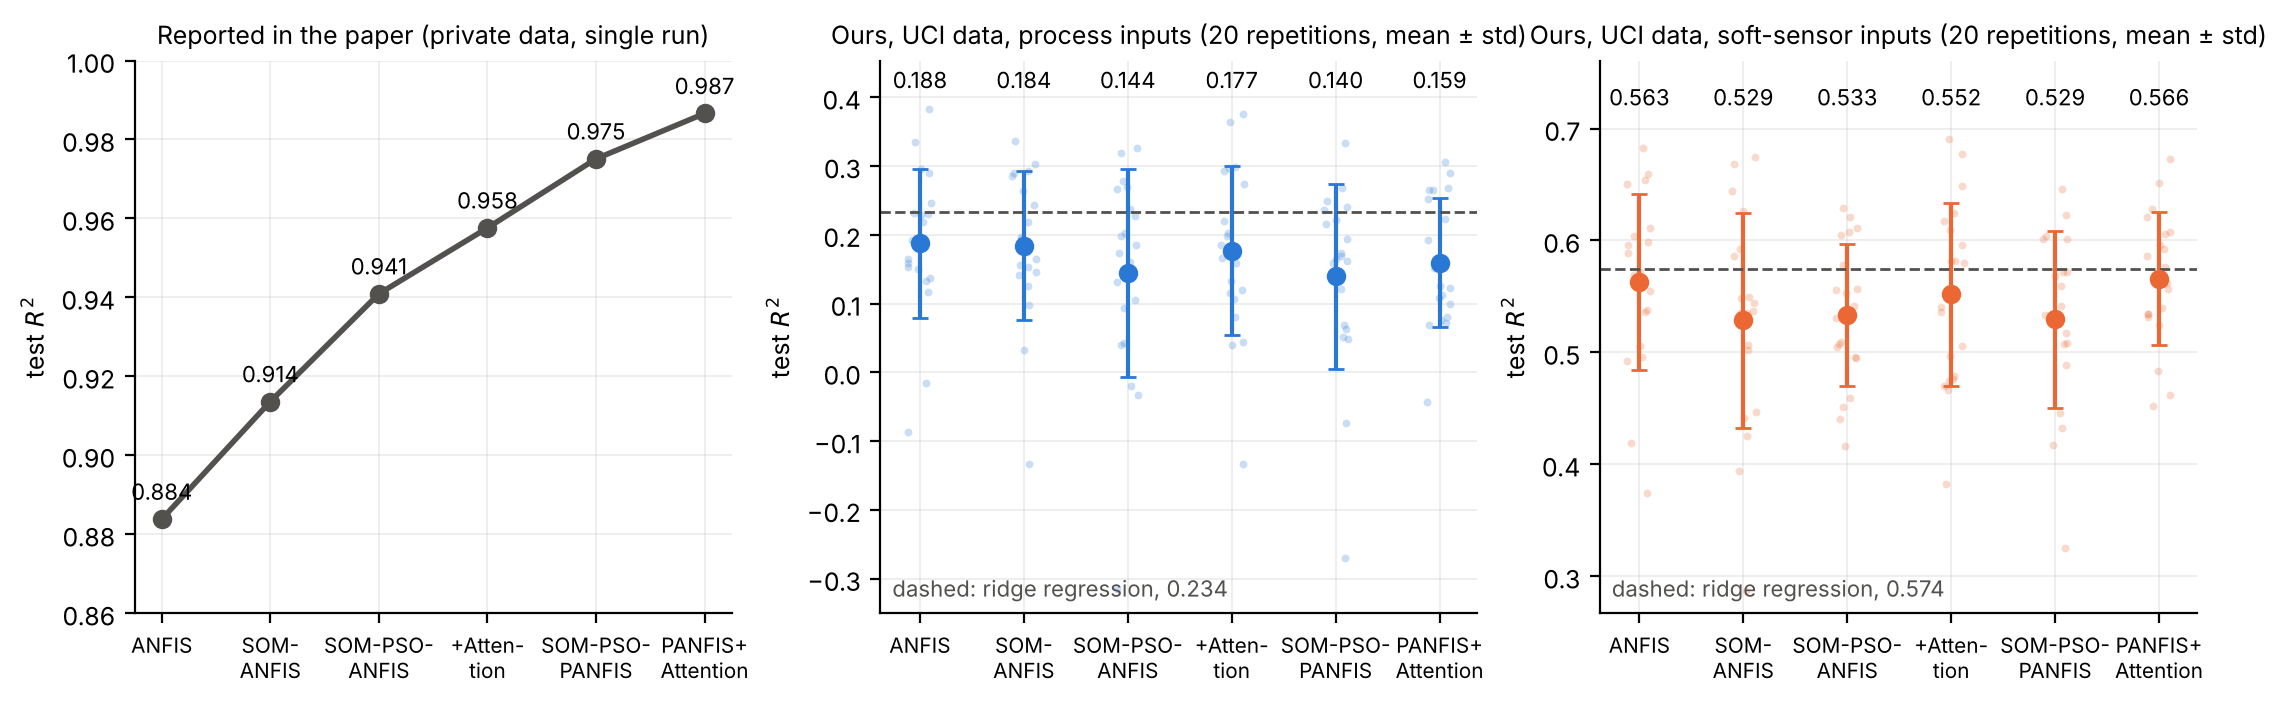
\includegraphics[width=\textwidth]{ladder.png}\\[1mm]
\small No step is statistically significant (all $p\ge0.11$, corrected resampled $t$-test); the signs alternate.
\end{frame}

\begin{frame}{Reproduction: numbers}
\centering\resizebox{0.86\textwidth}{!}{\tab{ladder_softsensor}}\\[2mm]
\small Soft-sensor inputs, 20 random splits. Ridge regression with 7 parameters matches the 13,238-parameter model.\\
Process inputs: full model is \emph{worse} than ridge ($\Delta R^2=-0.075$, $p=0.023$).
\end{frame}

\begin{frame}{Extension E1: which attention level matters?}
\begin{columns}[c]
\column{0.56\textwidth}
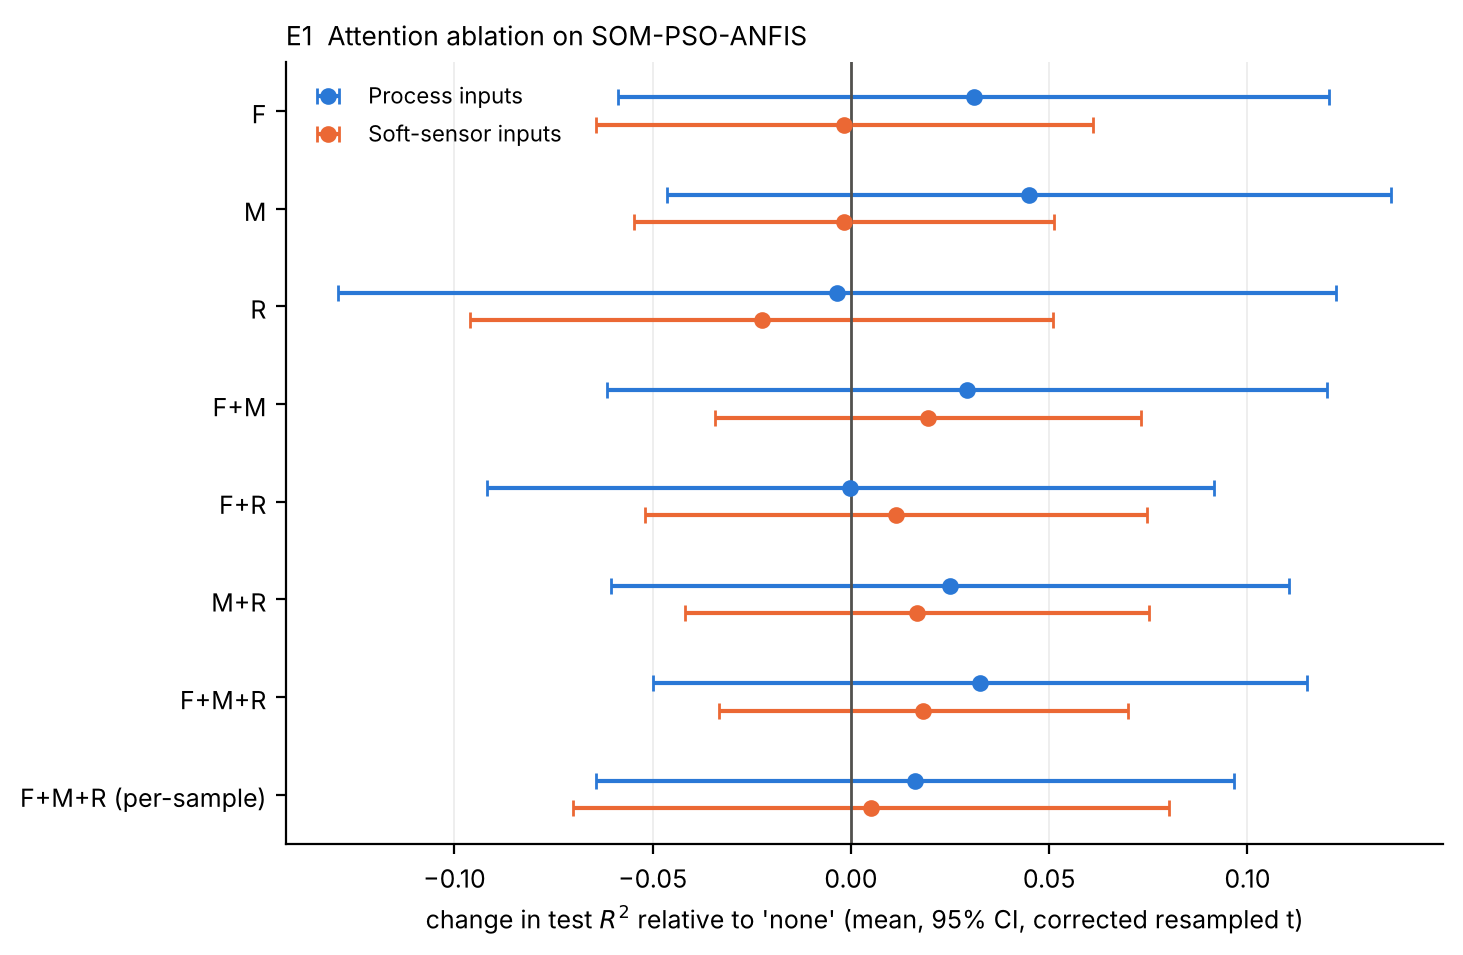
\includegraphics[width=\textwidth]{ablation.png}
\column{0.42\textwidth}
\begin{itemize}\setlength\itemsep{2mm}
\item all 8 subsets of \{Feature, MF, Rule\}
\item same split, same SOM + PSO start: only attention differs
\item every confidence interval includes zero
\item per-sample attention is not better
\item cost: 171 $\rightarrow$ 2,496 parameters
\end{itemize}
\end{columns}
\end{frame}

\begin{frame}{Extension E2: is PANFIS more than ``more rules''?}
\begin{columns}[c]
\column{0.56\textwidth}
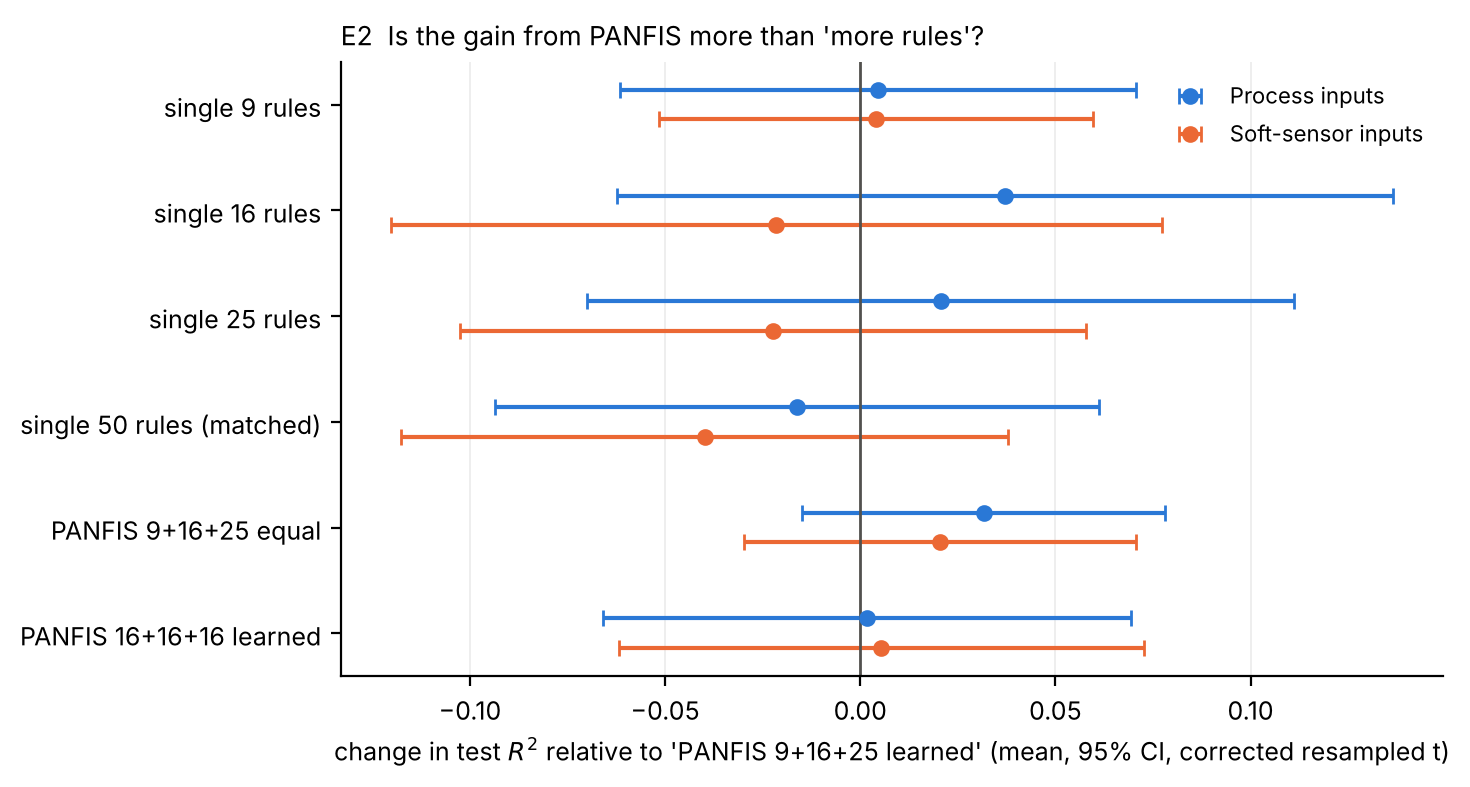
\includegraphics[width=\textwidth]{structure.png}
\column{0.42\textwidth}
\begin{itemize}\setlength\itemsep{2mm}
\item control the paper lacks: one ANFIS with 50 rules = same parameter count (950)
\item PANFIS vs.\ matched single model: not significant
\item 9 rules are as good as 50
\item equal fusion weights $\ge$ learned ones
\item 9+16+25 is no better than 16+16+16
\end{itemize}
\end{columns}
\end{frame}

\begin{frame}{Extensions E3 and E4: PSO fitness, noise robustness}
\begin{columns}[c]
\column{0.6\textwidth}
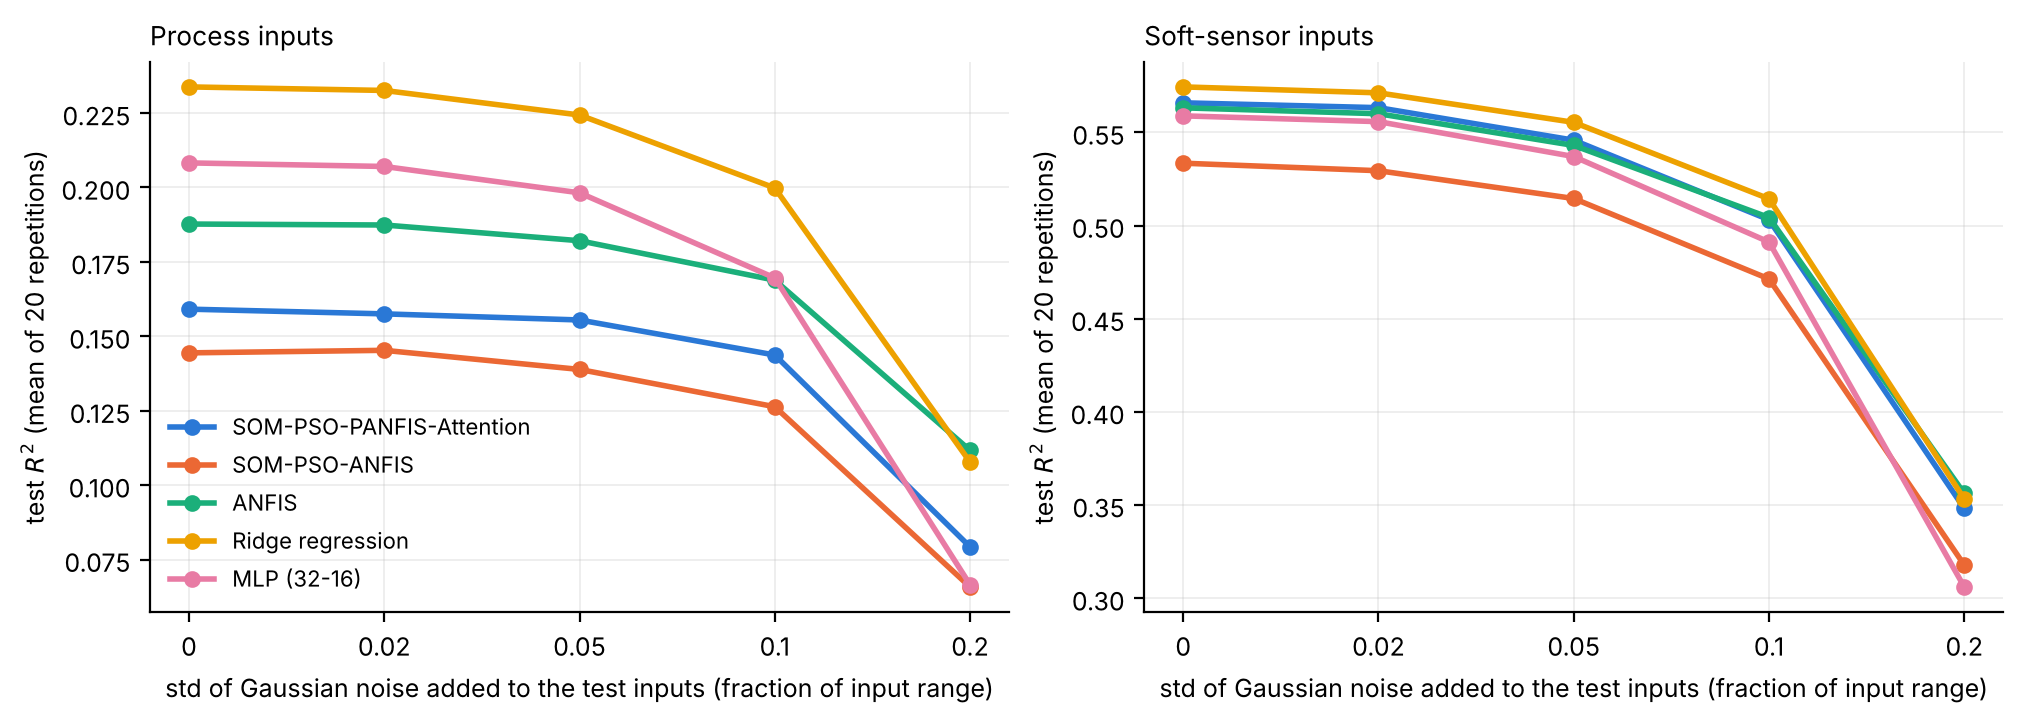
\includegraphics[width=\textwidth]{noise.png}
\column{0.38\textwidth}
\textbf{E3} PSO fitness on validation instead of training data: $+0.025$ / $+0.000$, not significant. No PSO at all is as good.\\[3mm]
\textbf{E4} Noise on the test inputs: all models degrade alike; attention and PANFIS do not add robustness.
\end{columns}
\end{frame}

\begin{frame}{Baseline vs.\ simplified model}
\begin{columns}[c]
\column{0.58\textwidth}
\resizebox{\linewidth}{!}{\tab{summary_baseline_vs_proposed}}
\column{0.38\textwidth}
\textbf{Baseline:} the paper's final model\\ (SOM-PSO-PANFIS-Attention)\\[2mm]
\textbf{Simplified:} PANFIS, equal weights, no attention\\[3mm]
Same accuracy within noise,\\ \textbf{93\% fewer parameters}.
\end{columns}
\end{frame}

\begin{frame}{Why? Discussion}
\begin{enumerate}\setlength\itemsep{3mm}
\item \textbf{Little non-linear signal.} A linear model is as good as a random forest on this data. A first-order Sugeno system already contains the linear model, so better membership functions cannot help.
\item \textbf{Small data.} 353 training samples against 171 to 13,238 parameters. Early stopping ends training before the membership functions move far. PSO lowers the \emph{training} error, which is not generalisation.
\item \textbf{Effects below the noise.} The paper's gains are 0.01--0.03 in \Rsq{}; the split-to-split spread here is 0.06--0.15. A single run cannot resolve them.
\end{enumerate}
\vspace{3mm}
What survives: the plain 9-rule ANFIS is \textbf{readable}: every prediction traces to a few rules in mg/L.
\end{frame}

\begin{frame}[fragile]{Live demo}
\small
\begin{verbatim}
python demo.py                              # typical day, SOM-PSO-ANFIS
python demo.py --set DBO-D=180 DQO-D=350    # change inputs
python demo.py --row 3 --model panfis-attention --scenario softsensor
\end{verbatim}
\normalsize
The script trains the model in a few seconds and prints, for the chosen input:
\begin{itemize}
\item crisp inputs and their scaled values
\item membership degree of every input in the strongest rules (layer 1)
\item normalised firing strength of each rule (layers 2--3)
\item the rule's linear consequent and its output in mg/L (layer 4)
\item the weighted average = predicted effluent BOD (layer 5)
\end{itemize}
\end{frame}

\begin{frame}{Limitations and conclusion}
\begin{columns}[T]
\column{0.48\textwidth}
\textbf{Limitations}
\begin{itemize}
\item private data of the paper unavailable: trends, not numbers
\item AutoGAN replaced by simple statistics
\item unspecified details filled in by me
\item small dataset, 75 test samples: effects under $\pm$0.05--0.1 undetectable
\item six inputs, paper's hyper-parameters
\end{itemize}
\column{0.48\textwidth}
\textbf{Conclusion}
\begin{itemize}
\item fuzzy core re-implemented and verified
\item on public data, no stage of the framework gives a significant gain; ridge regression is as accurate
\item attention and PANFIS add parameters, not accuracy
\item the paper's tables are inconsistent for its two best models
\end{itemize}
\end{columns}
\end{frame}
\end{document}
